\documentclass{article}
\usepackage[utf8]{inputenc}
\usepackage[english]{babel}
\usepackage[a4paper,top=3.5cm,bottom=3.5cm,left=3.5cm,right=3.5cm,%
bindingoffset=0mm]{geometry}
\usepackage{amssymb}
\usepackage{amsmath}
\newtheorem{prop}{Proposition}
\newtheorem{lemma}{Lemma}
\newenvironment{proof}[1][Proof]{\begin{trivlist}
		\item[\hskip \labelsep {\bfseries #1}]}{\end{trivlist}}
\newcommand{\qed}{\nobreak \ifvmode \relax \else
	\ifdim\lastskip<1.5em \hskip-\lastskip
	\hskip1.5em plus0em minus0.5em \fi \nobreak
	\vrule height0.75em width0.75em depth0em\fi}
\usepackage{tikz}
\usepackage{graphicx}
\usepackage{rotating}
\usepackage{float}
\linespread{1.3}
\raggedbottom




%
\font\reali=msbm10 at 12pt
% subsets of real numbers
\newcommand{\real}{\hbox{\reali R}}
\newcommand{\realp}{\hbox{\reali R}_{\scriptscriptstyle +}}
\newcommand{\realpp}{\hbox{\reali R}_{\scriptscriptstyle ++}}
\newcommand{\R}{\mathbb{R}}
\DeclareMathOperator{\E}{\mathbb{E}}
%

\title{First Draft}
\author{Marco Brianti\\Laura Gati}
\date{October 2017}


\begin{document}
	
	\maketitle
	
	\tableofcontents
	
	\section{Introduction}
	
	A hotly discussed current issue in the economics profession is the slow recovery of TFP after the Great Recession. A strand of literature in the wake of Comin and Gertler (2006) is highlighting that this slow recovery may be due to the endogenous component of TFP.\footnote{Such models capture a setting where TFP can be endogenously affected through R\&D expenditure. In this setting, a standard negative shock in exogenous TFP will imply not only a decrease in TFP itself via the exogenous component, but also a decrease in R\&D investment, due to the lack of resources in the economy. This decrease in R\&D investment leads to a decrease in the endogenous component of TFP. As a result, TFP overall will not only be lower than without the endogenous mechanism, but its lower level will start this process anew, thus triggering a negative spiral. Therefore the same negative technology shock will have both higher level and propagation effects.} Among these papers are Anzoategui et al. (2016), Bianchi et al. (2016) and Moran and Queralto (2017). However,  macroeconomic literature has expressed two major concerns with this interpretation: 1.) As clearly explored by Fernald, Hall, Stock and Watson (2017), the slowdown in TFP started in 2006, that is \emph{before} the financial crisis. 2.) R\&D triggers significant effects on TFP only after a remarkable amount of time, so it is hard to rationalize a decrease in R\&D at the time of the crisis as immediately leading to a slowdown in TFP. For these reasons, an explanation of the TFP slowdown merely based on lower R\&D investment cannot successfully explain how to relate these empirical facts to the models proposed in this literature, since in such models, the decrease in R\&D is due to a weak demand triggered by the financial crisis.
	
	In this project we aim to explain the slowdown in TFP using an endogenous growth model \`a la Comin and Gertler (2006), but, crucially, we aim to address the two main critiques pointed out above. Our model, therefore, shifts the focus from R\&D solely, to the role of expectations on more broad concepts of investment in endogenous TFP.
	
	As suggested by empirical papers such as Hall, Lotti, and Mairesse (2012), R\&D is not the only variable able to affect the endogenous component of TFP. In particular, investment in Information and Communication Techonlogy (hereafter IT investment) seems to be able to play an important role in driving the endogenous component of TFP. As an empirical motivation, in Figure 1 we show the log-levels of IT investment and the value of manufacturers new orders for IT industries (hereafter IT orders). Differently from R\&D expenditure, the slowdown of IT-related variables took place slightly before 2001 due to the burst of the IT bubble. Independently from the crisis, these variables never came back to the original trend and our aim is to assess the role of IT investment in the slowdown in TFP.
	
	\begin{figure}
		\centering
		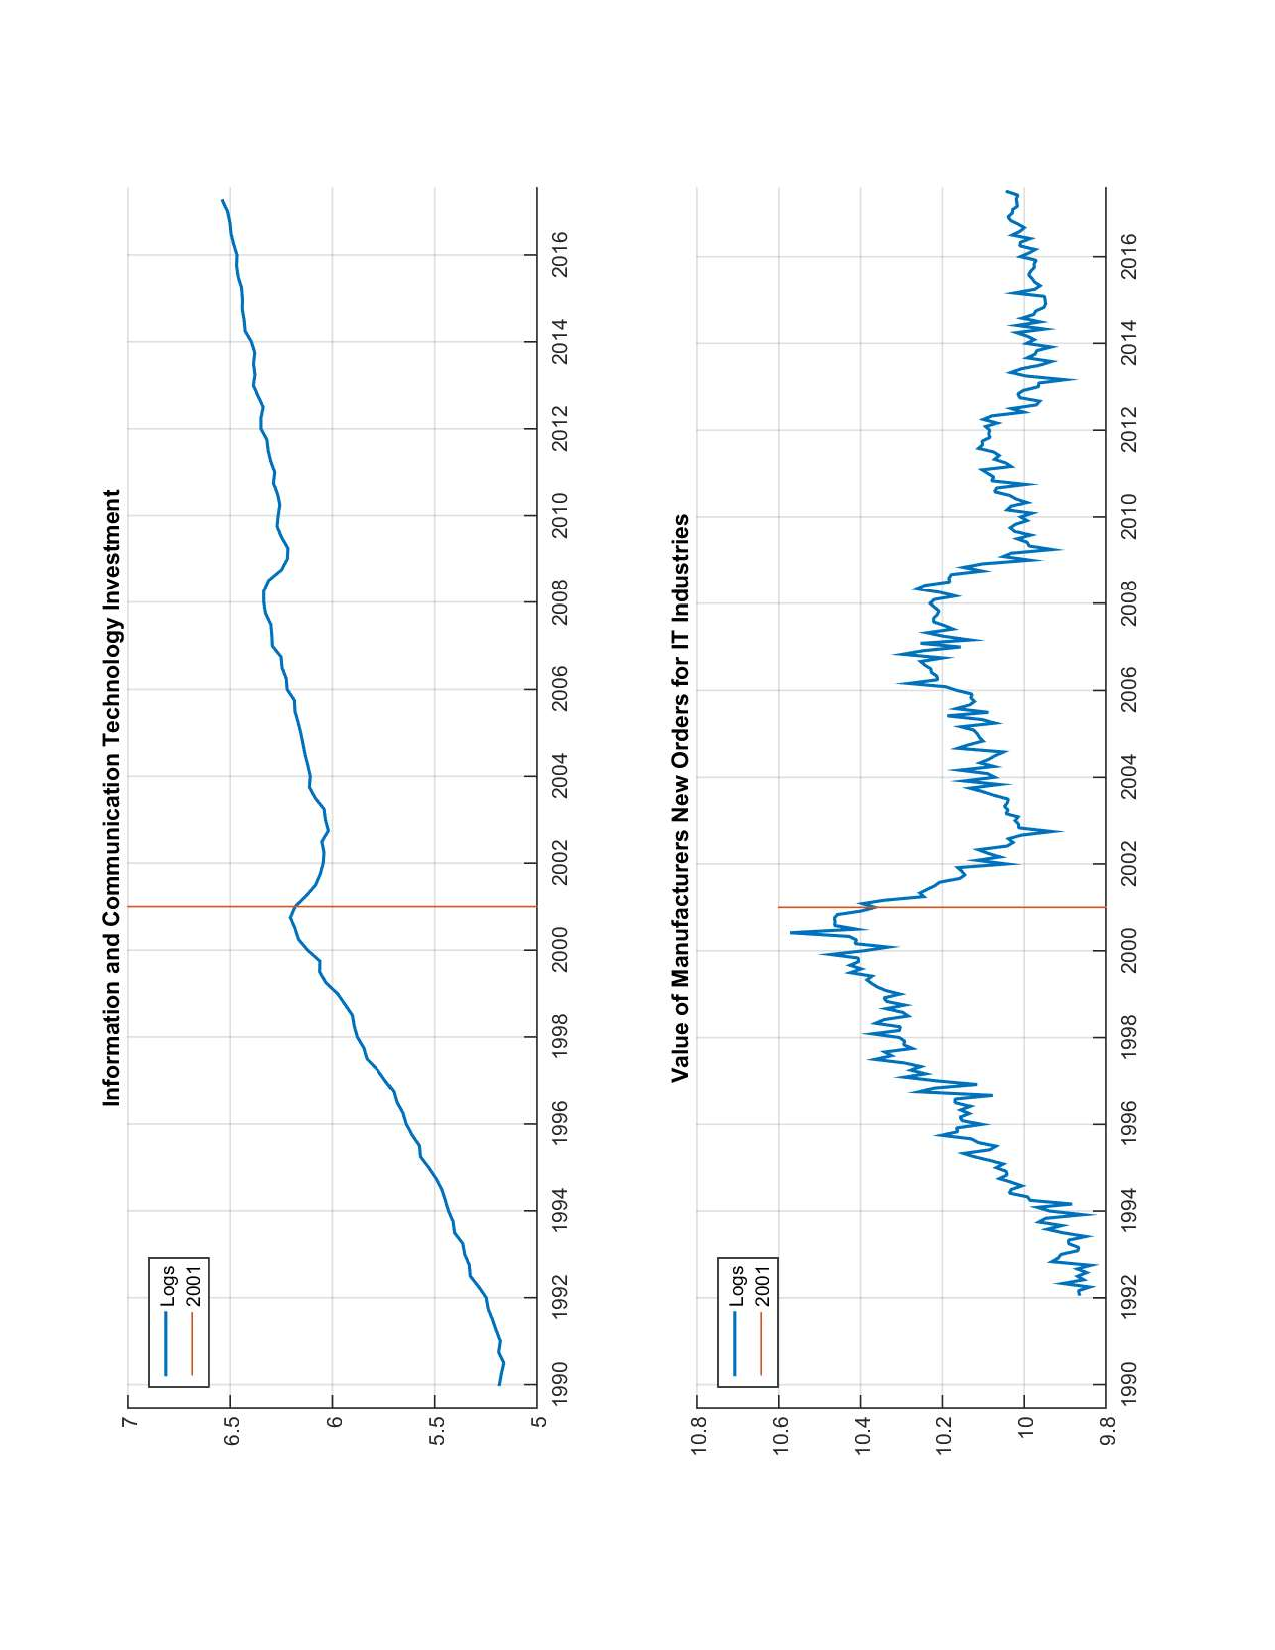
\includegraphics[scale=0.5, angle =270]{motivation}
		\caption{Data source is Federal Reserve Economic Data (FRED). IT investment is quarterly data and IT orders is monthly. Both variables are in log-levels.}
	\end{figure}	

A model that is postulating an endogenous determinant of TFP in the long run needs to take a stand on what sense this endogenous determinant differs from a news shock - the type of shock that in general is thought to be the driver of TFP in the long run. In particular, both of the shocks can be thought to happen contemporaneously but to be related to a future increase in TFP. Therefore, in order to be able to analyze these shocks separately we need to discipline our empirical and theoretical models to pin down a dimension of difference between them. 

The project is split into an empirical and theoretical part. The empirical part performs a structural VAR where we aim to identify news shocks as well as IT productivity shocks in a setting where TFP is endogenous. The theoretical part aims to provide a mechanism for the intuition that a news shock have a self-enforcing flavor through the endogenous component of TFP. As an example, assume that agents are hit by the exogenous signal that future TFP will be considerably higher. In this setting, due to fact that new ideas are more profitable when TFP is higher, a news shock will imply an increase in the perceived profitability of the IT sector, leading to a contemporaneous jump in this variable.\footnote{In particular, we subscribe to the interpretation of the IT investment process as a long-term investment whose results materialize with a lag. Following this logic, it is reasonable to believe that agents start to invest today in order to have new ideas ready to be sold when the expected jump in productivity actually arises.} Thus, a news shock implies a higher level of IT investment today which eventually will entail also a higher level of endogenous TFP in the future, confirming agents' expectations. Importantly, this mechanism does not rule out the existence of a completely exogenous news shock regarding the exogenous component of TFP but it considers the possibility that such a shock will naturally embody a mechanism of self-enforcing expectations.

\section{Empirical Evidence}

In this section, we follow a two-step procedure to investigate whether the mechanism outlined above is at work in the data. As a first step, we impose minimal discipline to simply bring together SVARs studied in the news shocks literature and in the endogenous TFP literature. Thus, the first VAR we run will be one that features both news shocks and IT productivity shocks, and we will impose only a minimal set of restrictions. This will be useful to get a first sense of the data and of how the system behaves when variables capturing news and endogenous TFP enter the system simultaneously. However, as we will explore in further detail below, this specification does not offer an adequate identification of news shocks in the presence of endogenous TFP, and thus also our IT productivity shocks may be poorly identified. Therefore, in a second step, we introduce an additional variable and impose a richer set of restrictions motivated by basic supply-demand theory to identify our shocks of interest.  

\subsection{First Set of Results}

\subsubsection{Specification and Identification Strategy}

Our first-step specification is the following 6-variable VAR 
\begin{equation}
\begin{pmatrix}
TFP_t \\ 
H_t \\
MI_{t+5|t} \\
IT_t \\
GDP_t \\
C_t \\
\end{pmatrix} = B(L) \begin{pmatrix}
TFP_{t-1} \\ 
H_{t-1} \\
MI_{t-1+5|t-1} \\
IT_{t-1} \\
GDP_{t-1} \\
C_{t-1} \\
\end{pmatrix} + i_t
\end{equation}
where $TFP_t$ is the log-level of Fernald total factor productivity, $H_{t}$ is the level of total number of hours worked, $MI_{t+5|t}$ is the level of Michigan Index of business confidence over 5 years, $IT_t$ is the log-level of IT investment, $GDP_t$ is the log-level of real gross domestic product, and $C_t$ is the log-level of real consumption. All the variables refer to the U.S. economy. $B(L)$ is a ($6\times 6$) matrix of lag-operator functions of the same order. In our favorite specification the order of the lag operator functions is two which implies that we regress variables at time $t$ with their own lagged values at $t-1$ and $t-2$. Finally, $i_t$ is a ($6\times 1$) vector of correlated innovations where $\Omega = i'_t i_t$.

In order to derive structural shocks $s_t$ from innovations $i_t$ we use a standard Cholesky identification strategy which imposes 15 zero-impact restrictions. Our identification strategy aims to identify a news shock and a IT productivity shock. In particular, we adhere to the following definitions of our shocks of interest. In line with the news shock literature, a news shock is defined as a signal regarding the future exogenous component of TFP.\footnote{In much of the news shock literature, this definition is not explicit in terms of \emph{exogenous} TFP, because in the absence of an endogenous TFP mechanism, exogenous TFP and total TFP are by definition the same object. Thus, defining a news shock as the shock that moves TFP over the long horizon implicitly amounts to saying that news move exogenous TFP.} The IT productivity shock (also IT shock) is by definition an increase in the sector-specific productivity that should lead to a natural increase in the IT level of investment. %Can we speak here about substitution effect?
The reason why we seek to identify also this second shock is because we want to disentangle the rise in IT investment given by an increase in the sector-specific productivity to the rise in IT investment due to future signals on exogenous TFP. %In other words, in order to size the self-enforcement effect of a news shock we need to disentangle the endogenous component embodied by an IT productivity shock, and, on the other hand, to correctly size the pure effect of an IT productivity shock we need to disentangle from IT its expectational component. 

In line with both strands of literature, we assume that both news shocks and IT productivity shocks have zero-impact effect on TFP. However, in order to distinguish these two, we impose a zero impact response of the Michigan Index to IT productivity shocks. We are using this last restriction in order to clean out any expectational effect from IT productivity shocks. In other words, an IT productivity shock should just show the effects of an unexpected and orthogonal increase in IT investment due to a contemporaneous shift in the sector-specific IT productivity, without embodying any hidden information regarding the future states of exogenous TFP. Failing to impose such a restriction will lead to upward-biased results on the effect of IT shocks on future TFP since we will not be able to distinguish between the exogenous news and the endogenous mechanism. However, on the other hand, we are not restricting the response of IT expenditure to news shocks since we are open to the idea that agents in response to a future increase in TFP will opt for a contemporaneous increase in IT investment. In particular, this is the self-enforcing behavior of the news shock that we are seeking to test.\footnote{As already argued, new technologies may be more profitable when TFP is higher, implying that a news shock would trigger an increase in the perceived profitability of the IT sector, leading to a contemporaneous jump in this variable.}

\subsection{Results}

In this subsection we present impulse response functions and variance decomposition of news shocks and IT productivity shocks. 

\begin{figure}[h!]
	\centering
	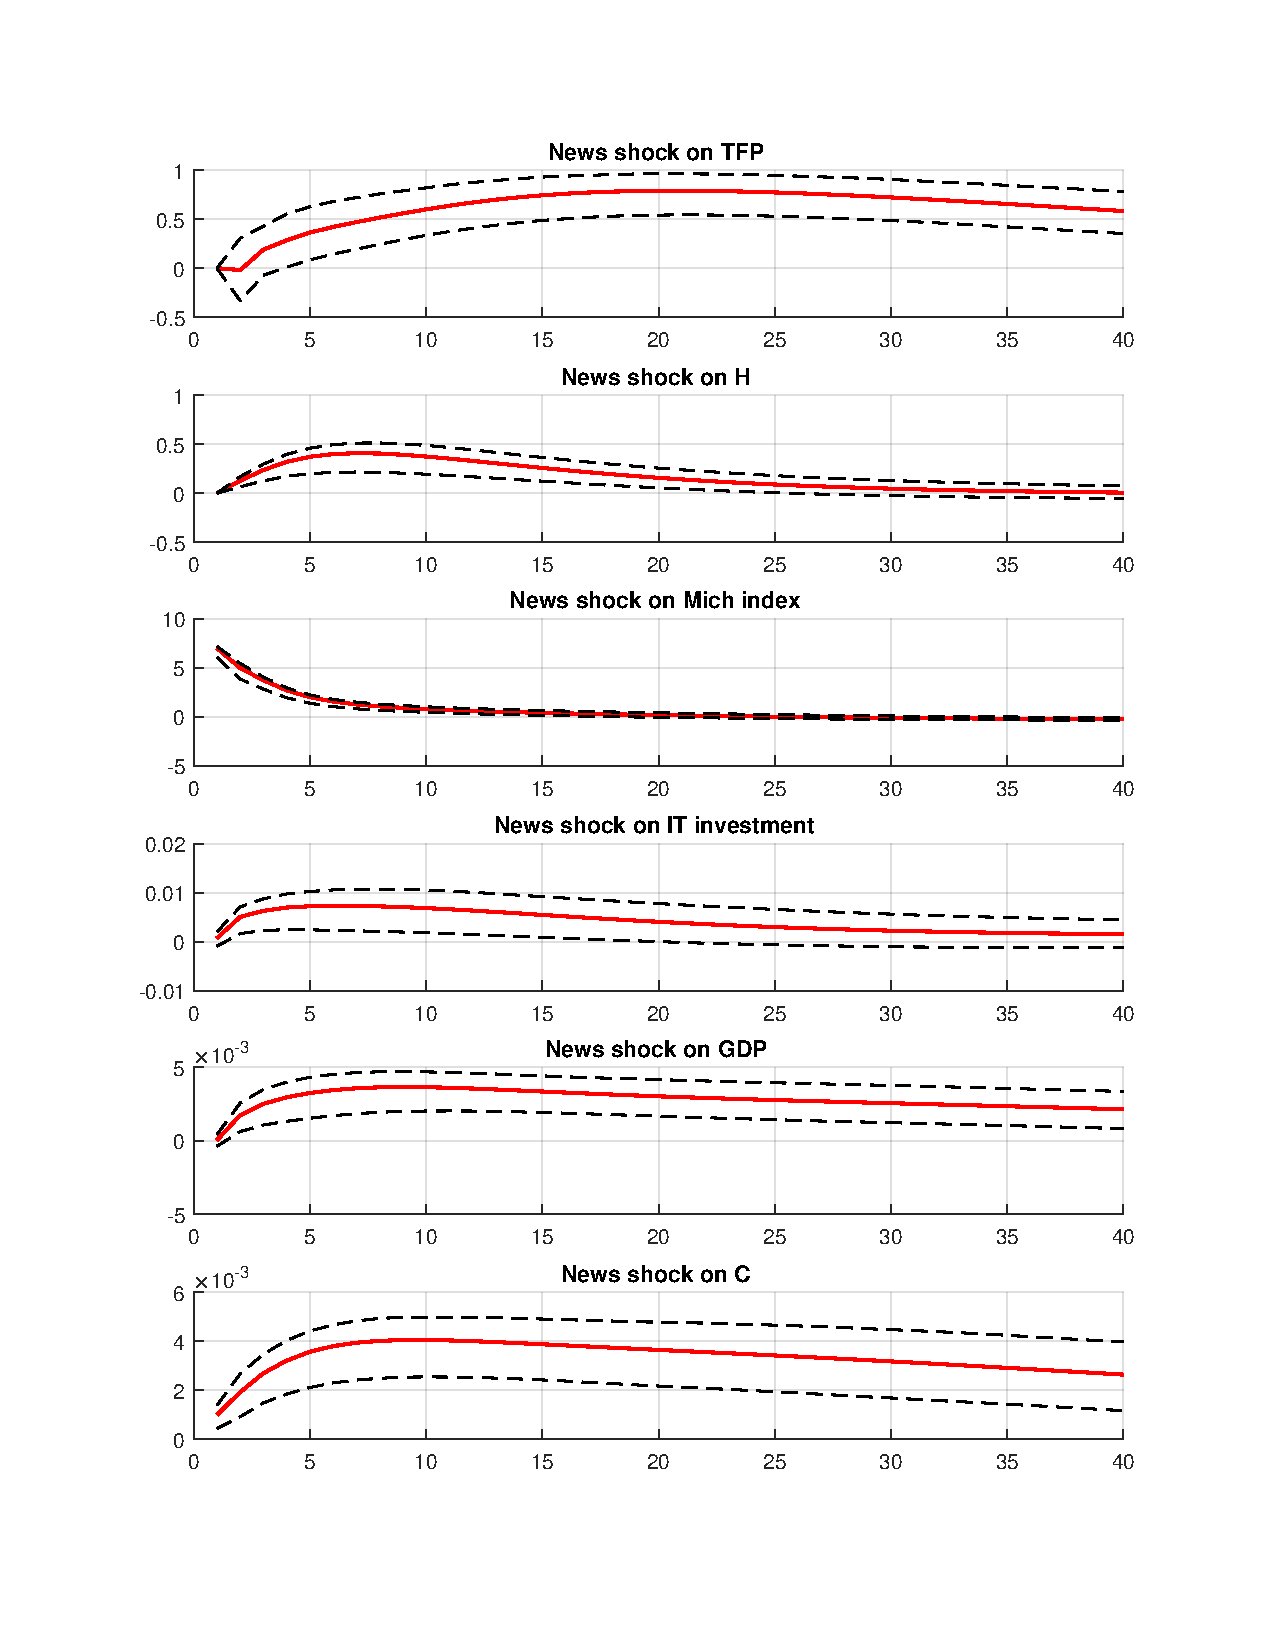
\includegraphics[scale=0.5]{figure(1)_IT}
	\caption{Impulse responses of aggregate macroeconomic variables to a news shock. Red solid line is point estimation and dashed lines are 90\% confidence intervals.}
\end{figure}
\begin{figure}
	\centering
	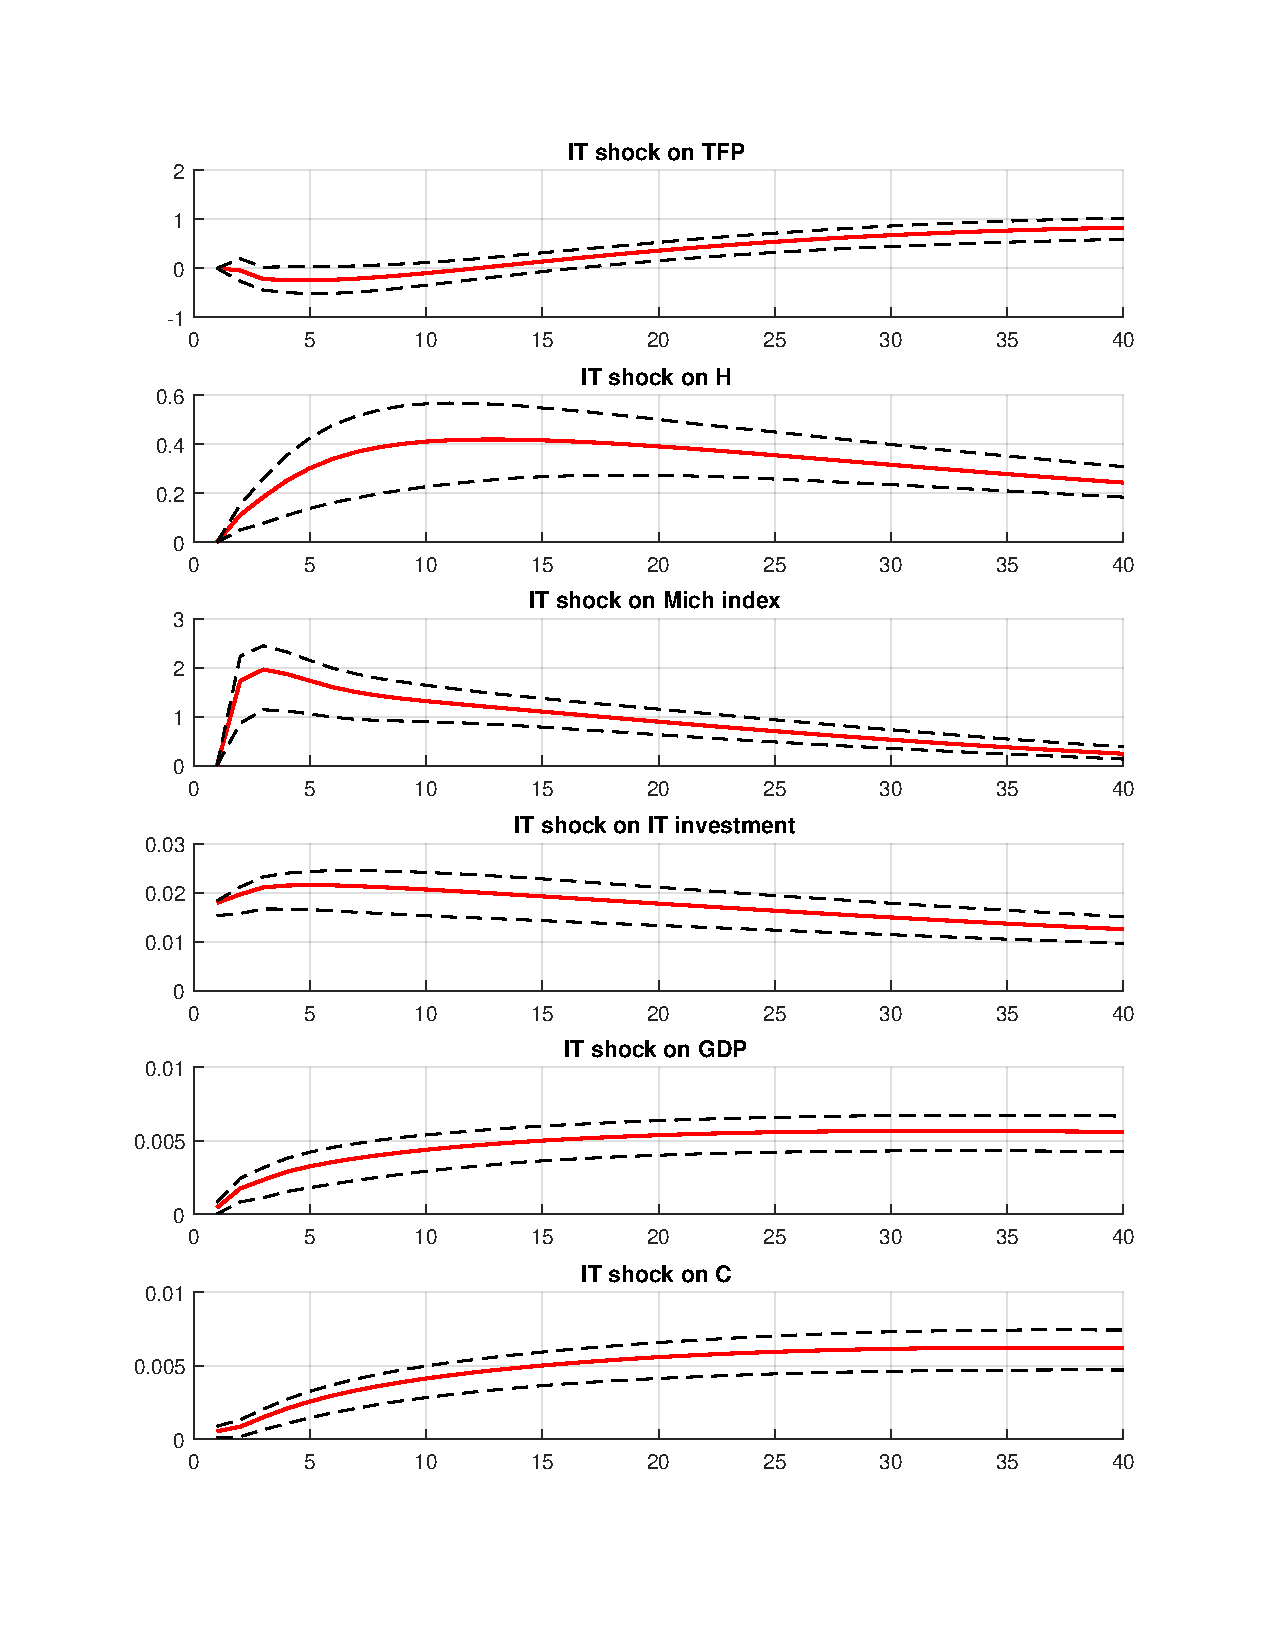
\includegraphics[scale=0.5]{figure(2)_IT}
	\caption{Impulse responses of aggregate macroeconomic variables to a IT shock. Red solid line is point estimation and dashed lines are 90\% confidence intervals.}
\end{figure}

\begin{table}[h!]
	\centering
	\begin{tabular}{ c c c }
		&       News shock     &      IT shock \\
		TFP              &       [    0.1733]   &      [  0.0990] \\
		H                &       [    0.0931]   &      [  0.2311] \\
		Mich index       &       [    0.5234]   &      [  0.2048] \\
		IT investment    &       [    0.0430]   &      [  0.6416] \\
		GDP              &       [    0.1406]   &      [  0.4178] \\
		C                &       [    0.1766]   &      [  0.4118] \\
	\end{tabular}
	%		\caption{Percentage variance explained by news shocks and IT shocks on TFP, hours worked, business confidence, information and technology investment, GDP, and consumption. The horizon is set to be 10 years.}\\
\end{table}

Our results from this specification are broadly in line with the two strands of literature we're bringing together. Considering first the impulse responses following a news shock, we see a delayed positive effect on TFP. In particular, it is significant after five quarters and, although diminishing, its effect is still positive after 10 years. As expected, news have a significant impact effect on agents' expectations as proxied by the Michigan index of business confidence over 5 years. In addition, news have a small but positive impact effect on consumption, investment in IT and economic outcome.

This effect gradually gets larger for all the variables, mirroring the response of TFP. Specifically, we are interested in the positive and prolonged response of IT investment which suggests a self-enforcing behavior of news in the economy.

Interestingly, an IT shock has a even more delayed effect on TFP. In line with the related empirical literature, an improvement in the IT sector takes almost 5 years to trigger an effect on TFP. Additionally, IT shocks have a sharp and positive effect on agents' confidence after the zero-impact restriction.\footnote{This sharp response of agents' expectations after the zero-impact restriction is a fair critique to our identification strategy, as it suggests a problem of reverse causality between news and IT efficiency. This is the reason we attempt a more disciplined identification strategy in the next section.} Due to the shift in IT productivity, IT investment has a positive response for a prolonged period of time confirming the importance of this shock on economic activity. Moreover, consumption and GDP have a slightly delayed positive response which increases over time and remains high even after 10 years.

Finally, focusing on Table 1, news explain almost 20\% of the variance of TFP over a 10-year horizon. Alternatively, a IT productivity shock is able to explain almost the 10\% over the same horizon. Although, news shocks seem to be able to better explain TFP in the long run, IT shocks have a more important effect on real variables like hours worked, consumption, and GDP over 10 years.


\subsubsection{Concerns}


As discussed in the previous sections, there are several reasons to be concerned that our first specification does not adequately disentangle news shocks from IT shocks. The short-run identification strategy followed in the previous section assumes the same zero impact effect on TFP both from news and IT shocks. The only restriction that imposes any difference between the two shocks is that the variable capturing news, the Michigan index, should not react on impact to an IT shock. The entire validity of the procedure hinges on whether this assumption is sufficient to neatly disentangle the two shocks.

However, there are ample reasons for why this might not be the case. First of all, as noted above, the response of the Michigan index to an IT shock shoots into significant territory immediately after impact. Potentially, this reflects that the zero-impact restriction may be not enough to clean out expectational effects from the IT shock which is suggestive of the fact that identified IT shocks may embody a part of news biasing the effects and relevance of an IT shock. In other words, an IT shock identified using the Cholesky procedure cannot pin down an \emph{exogenous} sector-specific IT productivity shock, but a convex combination between itself and news. Then, it means that with these procedure we are also biasing the effects and relevance of news since a part of it is incorrectly shifted to IT shocks. As a result,  zero-impact restrictions are not sufficient to distinguish between news and IT suggesting the need for an improved identification strategy.



\subsection{A Second Identification Strategy}

%Attempt to fully cleaning a sector-specific IT productivity shock from a signal on the exogenous component of TFP.
In order to tackle the challenges presented above, we propose a second identification strategy that relies on basic supply-demand theory from macroeconomics to pin down other observable differences between news and IT shocks. The idea is the following. 

Inside the specific IT sector, a news shock resembles the same effects of a demand shock. In particular, IT productivity is completely unchanged but its demand is now stronger for the novel information that future TFP will be higher. This shift in the demand for IT items is likely due to a spillover effect that new technologies are more profitable when TFP is higher. Thus, in terms of nominal quantities, since news shocks look like sectoral demand shocks, we expect a contemporaneous increase in the sectoral prices. On the other hand, IT shocks imply supply-side changes in the IT sector, since the sector becomes more productive on impact. Thus, within the IT sector, the IT shock resembles supply shocks, involving sinking sectoral prices. Thus simple supply-demand theory gives us a dimension along which news shocks and IT shocks differ: they move prices in the IT sector in opposite directions.

In particular, in order to avoid having to deal with the general effect of both shocks on inflation, we will consider the relative price of IT, as given by the ratio $\frac{P^{IT}}{P}$, where $P$ is simply the CPI.\footnote{The reason we consider the relative price of IT is in general to avoid having to take a stance on the direction of price movements per se. In particular, a robust empirical finding of the news literature is that prices tend to decrease after a news shock. Thus, the prediction of supply-demand theory would be annulled in a framework where we only consider prices, while it remains operative if we take into account that prices across the board may be going down, but IT prices move less than prices of other items in the CPI.}

To spell out the identification strategy we derive from this line of thought, it is useful to consider a simple, reduced-form decomposition of the channels that determine productivity:

\begin{equation}
TFP_t =  \underbrace{\varepsilon_t}_\text{surprise tech shock}  + \underbrace{\underbrace{V_{t-1}}_\text{news shock} + \underbrace{IT_{t-1}}_\text{\text{IT shock}}}_\text{$N_{t-1}$}  \\
\end{equation}

Equation (2) illustrates that in the model we have in mind, the productivity of the economy is governed by three forces: contemporaneous shocks to exogenous TFP, news shocks that exogenously affect productivity with a lag, and IT shocks that endogenously affect productivity with a lag. Note that defining $N_{t-1} = V_{t-1} + IT_{t-1}$ would yield the specification of Barsky \& Sims, where productivity is thought of as driven by surprise shocks to technology and a news shock, $N_{t-1}$. Barsky and Sims (2011) identify $N_{t-1}$ as the shock that maximizes the forecast error variance (FEV) of TFP in the long run, thus capturing all the fluctuations in future TFP related to contemporaneous shocks. %$\varepsilon_t$ is simply considered as a reduced-form residual. 
This suggests that we can rely on a combination of the Barsky and Sims (2011) strategy and the implications of supply-demand theory to simultaneously identify our news shock, $V_{t-1}$, and our IT shock, $IT_{t-1}$. In particular, our second identification strategy can be summarized as the following algorithm:

\begin{enumerate}
	\item The news shock $V_{t-1}$ maximizes the FEV of future TFP subject to the restriction that it has no effect on the relative price $\frac{P^{IT}}{P}$ in the long run;
	\item The IT shock maximizes the remaining FEV of future TFP.
    \item The tech shock $\varepsilon_t$ is considered as a residual shock and is left unrestricted;
\end{enumerate}


\subsection{Second Set of Results}

We still need to implement this identification strategy. 


\end{document}
